
\QCMautoevaluation{Pour chaque question, plusieurs réponses sont
  proposées.  Déterminer celles qui sont correctes.}

\begin{QCM}
  \begin{GroupeQCM}
  
      \begin{center} 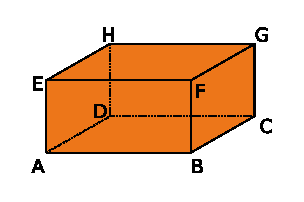
\includegraphics[width=4.5cm]{paveABCDEFGH} \end{center}
      \begin{center} $ABCDEFGH$ est un pavé droit. \end{center}
      
    \begin{exercice}
      \begin{ChoixQCM}{4}
      \item $[HD]$ est une arête
      \item $[EF]$ est une arête
      \item $[BG]$ est une arête
      \item $[AG]$ est une arête
      \end{ChoixQCM}
\begin{corrige}
     \reponseQCM{ab}
   \end{corrige}
    \end{exercice}
    
    \begin{exercice}
      \begin{ChoixQCM}{4}
      \item La longueur $EA$  sur la figure est en vraie grandeur
      \item La longueur $FG$  sur la figure est en vraie grandeur
      \item La longueur $FC$  sur la figure est en vraie grandeur
      \item La longueur $HC$  sur la figure est en vraie grandeur
      \end{ChoixQCM}
\begin{corrige}
     \reponseQCM{ad}
   \end{corrige}
    \end{exercice}
    
    
     \begin{exercice}
      \begin{ChoixQCM}{4}
      \item Les faces $ABCD$ et $AEFB$ sont parallèles
      \item Les faces $ABCD$ et $EFGH$ sont parallèles
      \item Les faces $EADH$ et $FBCG$ sont parallèles
      \item Les faces $EADH$ et $EFGH$ sont parallèles
      \end{ChoixQCM}
\begin{corrige}
     \reponseQCM{bc}
   \end{corrige}
    \end{exercice}
    
    
     \begin{exercice}
      \begin{ChoixQCM}{4}
      \item $AB = EF = HG$
      \item $FG = EF$
      \item $EH = AD = HG$
      \item $HD = EA = FB$
      \end{ChoixQCM}
\begin{corrige}
     \reponseQCM{ad}
   \end{corrige}
    \end{exercice}
    
    
     \begin{exercice}
      \begin{ChoixQCM}{4}
      \item $(AD)$ est perpendiculaire à $(AB)$
      \item $(AD)$ et $(BC)$ sont parallèles
      \item $(AD)$ et $(DC)$ sont parallèles
      \item $(AD)$ est perpendiculaire à $(HD)$
      \end{ChoixQCM}
\begin{corrige}
     \reponseQCM{abd}
   \end{corrige}
    \end{exercice}
    
    
     \begin{exercice}
      \begin{ChoixQCM}{4}
      \item $FBC$ est équilatéral
      \item $FHE$ est isocèle en $F$
      \item $BCD$ est quelconque
      \item $FBC$ est rectangle en $B$
      \end{ChoixQCM}
\begin{corrige}
     \reponseQCM{d}
   \end{corrige}
    \end{exercice}

    
    \begin{exercice}
      Le pavé ABCDEFGH a pour patron(s) possible(s) \ldots
      \begin{ChoixQCM}{4}
      \item 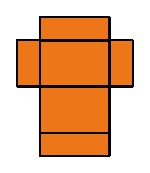
\includegraphics[width=2cm]{ABCDEFGH_patron1}
      \item 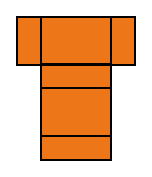
\includegraphics[width=2cm]{ABCDEFGH_patron2}
      \item 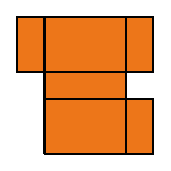
\includegraphics[width=2cm]{ABCDEFGH_patron3}
      \item 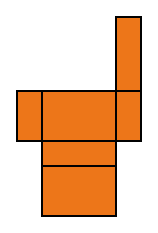
\includegraphics[width=2cm]{ABCDEFGH_patron4}
      \end{ChoixQCM}
\begin{corrige}
     \reponseQCM{abd}
   \end{corrige}
    \end{exercice}
 \end{GroupeQCM}
\end{QCM}   
    
    
\begin{QCM}
  \begin{GroupeQCM}
      
    \begin{exercice}
      Le volume d'un cube de 3 cm d'arête est \ldots
      \begin{ChoixQCM}{4}
      \item 3 cm\up{3}
      \item 9 cm\up{3}
      \item 27 cm\up{3}
      \item 12 cm\up{3}
      \end{ChoixQCM}
\begin{corrige}
     \reponseQCM{c}
   \end{corrige}
    \end{exercice}


    \begin{exercice}
      Quelle phrase est vraie ?
      \begin{ChoixQCM}{4}
      \item Si on double la longueur de l'arête d'un cube alors son volume double aussi
      \item Si on double la longueur de l'arête d'un cube alors son volume est multiplié par 4
      \item Si on double la longueur de l'arête d'un cube alors son volume est multiplié par 8
      \item Si on double la longueur de l'arête d'un cube alors son volume est multiplié par 16
      \end{ChoixQCM}
\begin{corrige}
     \reponseQCM{c}
   \end{corrige}
    \end{exercice}
    
    
    \begin{exercice}
      Mon volume est de 12 cm\up{3} et la longueur totale de mes arêtes est de 28 cm. Qui puis‑je être ?
      \begin{ChoixQCM}{4}
      \item Je suis un pavé de dimensions  2 ; 2 et 3 en centimètres
      \item Je suis un cube d'arête 3 cm
      \item Je suis un pavé de dimensions 2 ; 7 et 2 en centimètres
      \item Je suis un pavé de dimensions  6 ; 2 et 1 en centimètres
      \end{ChoixQCM}
\begin{corrige}
     \reponseQCM{a}
   \end{corrige}
    \end{exercice}


\end{GroupeQCM}
\end{QCM}

  
